\section[Udviklingsmetode]{Udviklingsmetode}

% Emneoverskrift. Start jeres del med denne:
\begin{frame}
  \frametitle{}
  \begin{center}
    {\Huge Udviklingsmetode}
  \end{center}
\end{frame}
\note{
  \begin{itemize}
		\item Notes...
  \end{itemize}
}

\begin{frame}
    \frametitle{Udviklingsmetode i multiprojektet}
    \centering
    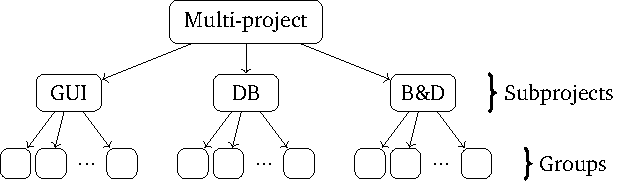
\includegraphics[width=0.8\textwidth]{multiproject_illustration.pdf}
\end{frame}
\note{
	\begin{itemize}
    \item \textbf{Unik struktur}. Vi ønsker at \textbf{tilfredsstille} kunden, men har også andre \textbf{prioriteter} såsom gode, indholdsrige emner, så \textbf{rapport} og \textbf{karakter} bliver gode.
    \item Vi kan ikke \textbf{fyre }grupper, \textbf{ingen autoritet}.
    \item Vi har valgt: \textbf{Scrum of Scrums} i 3 niveauer
    \item \textbf{AGIL} METODE godt valg:
    \begin{itemize}
      \item ingen \textbf{udvikler-erfaring} med kode + krav + kunder
      \item \textbf{Kun 4 måneder} > ikke tid til at forstå kodebasen
      \item Vi skal bruge tiden på at få den til at virke!
    \end{itemize}
    \item Scrum ca. 7 mand. \textbf{2 niveauer}: 15 mand
    \begin{itemize}
      \item Multiprojekt: Sikre at roller, work products og møderne overholdes.
      \item Subprojekt: Sprint planning, sprint review, og internt løse større problemer.
      \item Gruppe: Scrum of (something). Grupperne skal implementere interfacet Scrum. Samarbejde user stories input, estimering mm.
    \end{itemize}
	\end{itemize}
}

\begin{frame}
    \frametitle{Udviklingsmetode i multiprojektet}
    \framesubtitle{Typer af backlog items}
      \begin{mtjbox}[backgroundcolor=color1!5, linecolor=color1!40]
        Backlog Items
        \begin{columns}
          \begin{column}{0.48\textwidth}
            \begin{mtjbox}
              Feature (+ bug)
            \end{mtjbox}
          \end{column}
          \begin{column}{0.48\textwidth}
            \begin{mtjbox}
              Constraint
            \end{mtjbox}
          \end{column}
        \end{columns}

        \begin{columns}
          \begin{column}{0.48\textwidth}
            \begin{mtjbox}
              Knowledge Acquisition
            \end{mtjbox}
          \end{column}
          \begin{column}{0.48\textwidth}
            \begin{mtjbox}
              Technical Work
            \end{mtjbox}
          \end{column}
        \end{columns}
      \end{mtjbox}

\end{frame}
\note{
	\begin{itemize}
    \item \textbf{Vi startede} med 1 type: USER STORIES
    \item \textbf{Kritik} fra en anden gruppe: \textbf{Svært at formulere}, prioritere og arbejde på technical work, og knowledge acquisition.
    \item \textbf{Revidering}, databasegrupperne (technical work)
    \item \textbf{Feature/bug}: funktionelle krav, værdi for kunden. Både features og bugs er \textbf{noget kunden ønsker}, som ikke er der pt.
    \item \textbf{Constraint}: non-funktionelle krav, ikke tvinge ind i user story. Skrives på bagside, eller egen post-it.
    \item \textbf{Knowledge Acquisition}: Undersøge ting. Timeboxing muligt: spike fra XP.
    \item \textbf{Technical Work}: Vigtige opgaver for os udviklere (system+refactoring).

	\end{itemize}
}

\begin{frame}
    \frametitle{Udviklingsmetode i multiprojektet}
    \centering
    \StickyNoteFront{\ECFAugie{} \small As a <\emph{type of user}>,\\I want <\emph{some goal}>\\so that <\emph{some reason}>}
    ~~~~~~~
    \StickyNoteBack{\ECFAugie{} \small Conditions of satisfaction} % for sjov font
\end{frame}
\note{
  \begin{itemize}
    \item Før havde vi ikke en fast måde at skrive user stories.
    \item Revidering:
    \item Formulering konsekvent: nemmere at sammenligne, mere sigende.
    \item As a <type of user>, I want <some goal> so that <some reason>.
    \begin{itemize}
      \item ``type of user'' kan være udvikler, slutbruger eller andet.
    \end{itemize}
  \end{itemize}
}

\begin{frame}
    \note{
      \begin{itemize}
        \item Scrum master: \textbf{os}, som følge af \textbf{ansvar} for udviklingsmetode.
        \begin{itemize}
          \item Scrum Master for alle projektgrupper.
          \item \textbf{Overser metoder}
          \item \textbf{Guider} grupperne til at følge Scrum
        \end{itemize}
        \item Product owner: Skal \textbf{kende kundernes behov}, kontakt med kunder.
        \begin{itemize}
          \item \textbf{I starten}: 1 sprint review møde med eksterne kunder.
          \item Semesterkoordinator: kunderne er \textbf{ligeglade} med interne ting.
          \item \textbf{Løsning}: 3 sprint reviews. GUI speciel (kunde)
          \item I den forbindelse overvejede vi noget af \textbf{strukturen} i Scrum-of-Scrums.
          \item \textbf{Løsning}: Et subprojekt har egen product owner, kunde og backlog.
          \item ~~~~ Grupper kan være kunder for grupper.
          \item Figur: GUI har eksterne kunder som kunder. Resten har GUI og hinanden som kunder.
        \end{itemize}
      \end{itemize}
    }
    \frametitle{Udviklingsmetode i multiprojektet}
    \framesubtitle{Roller}
    \begin{columns}[t]
    \column{.5\textwidth}
      \begin{mdframed}[align=center, backgroundcolor=color3!10, linecolor=color3!50, linewidth=1pt]
        Scrum Master
      \end{mdframed}
    \column{.5\textwidth}
      \begin{mdframed}[align=center, backgroundcolor=color3!10, linecolor=color3!50, linewidth=1pt]
        Product Owner
      \end{mdframed}
      \vspace{.6cm}
      \centering
      \pause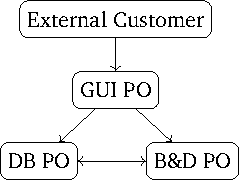
\includegraphics[width=.65\textwidth]{po_illustration.pdf}
    \end{columns}
\end{frame}



% Indhold:
\begin{frame}
    \frametitle{Udviklingsmetode i vores gruppe}
    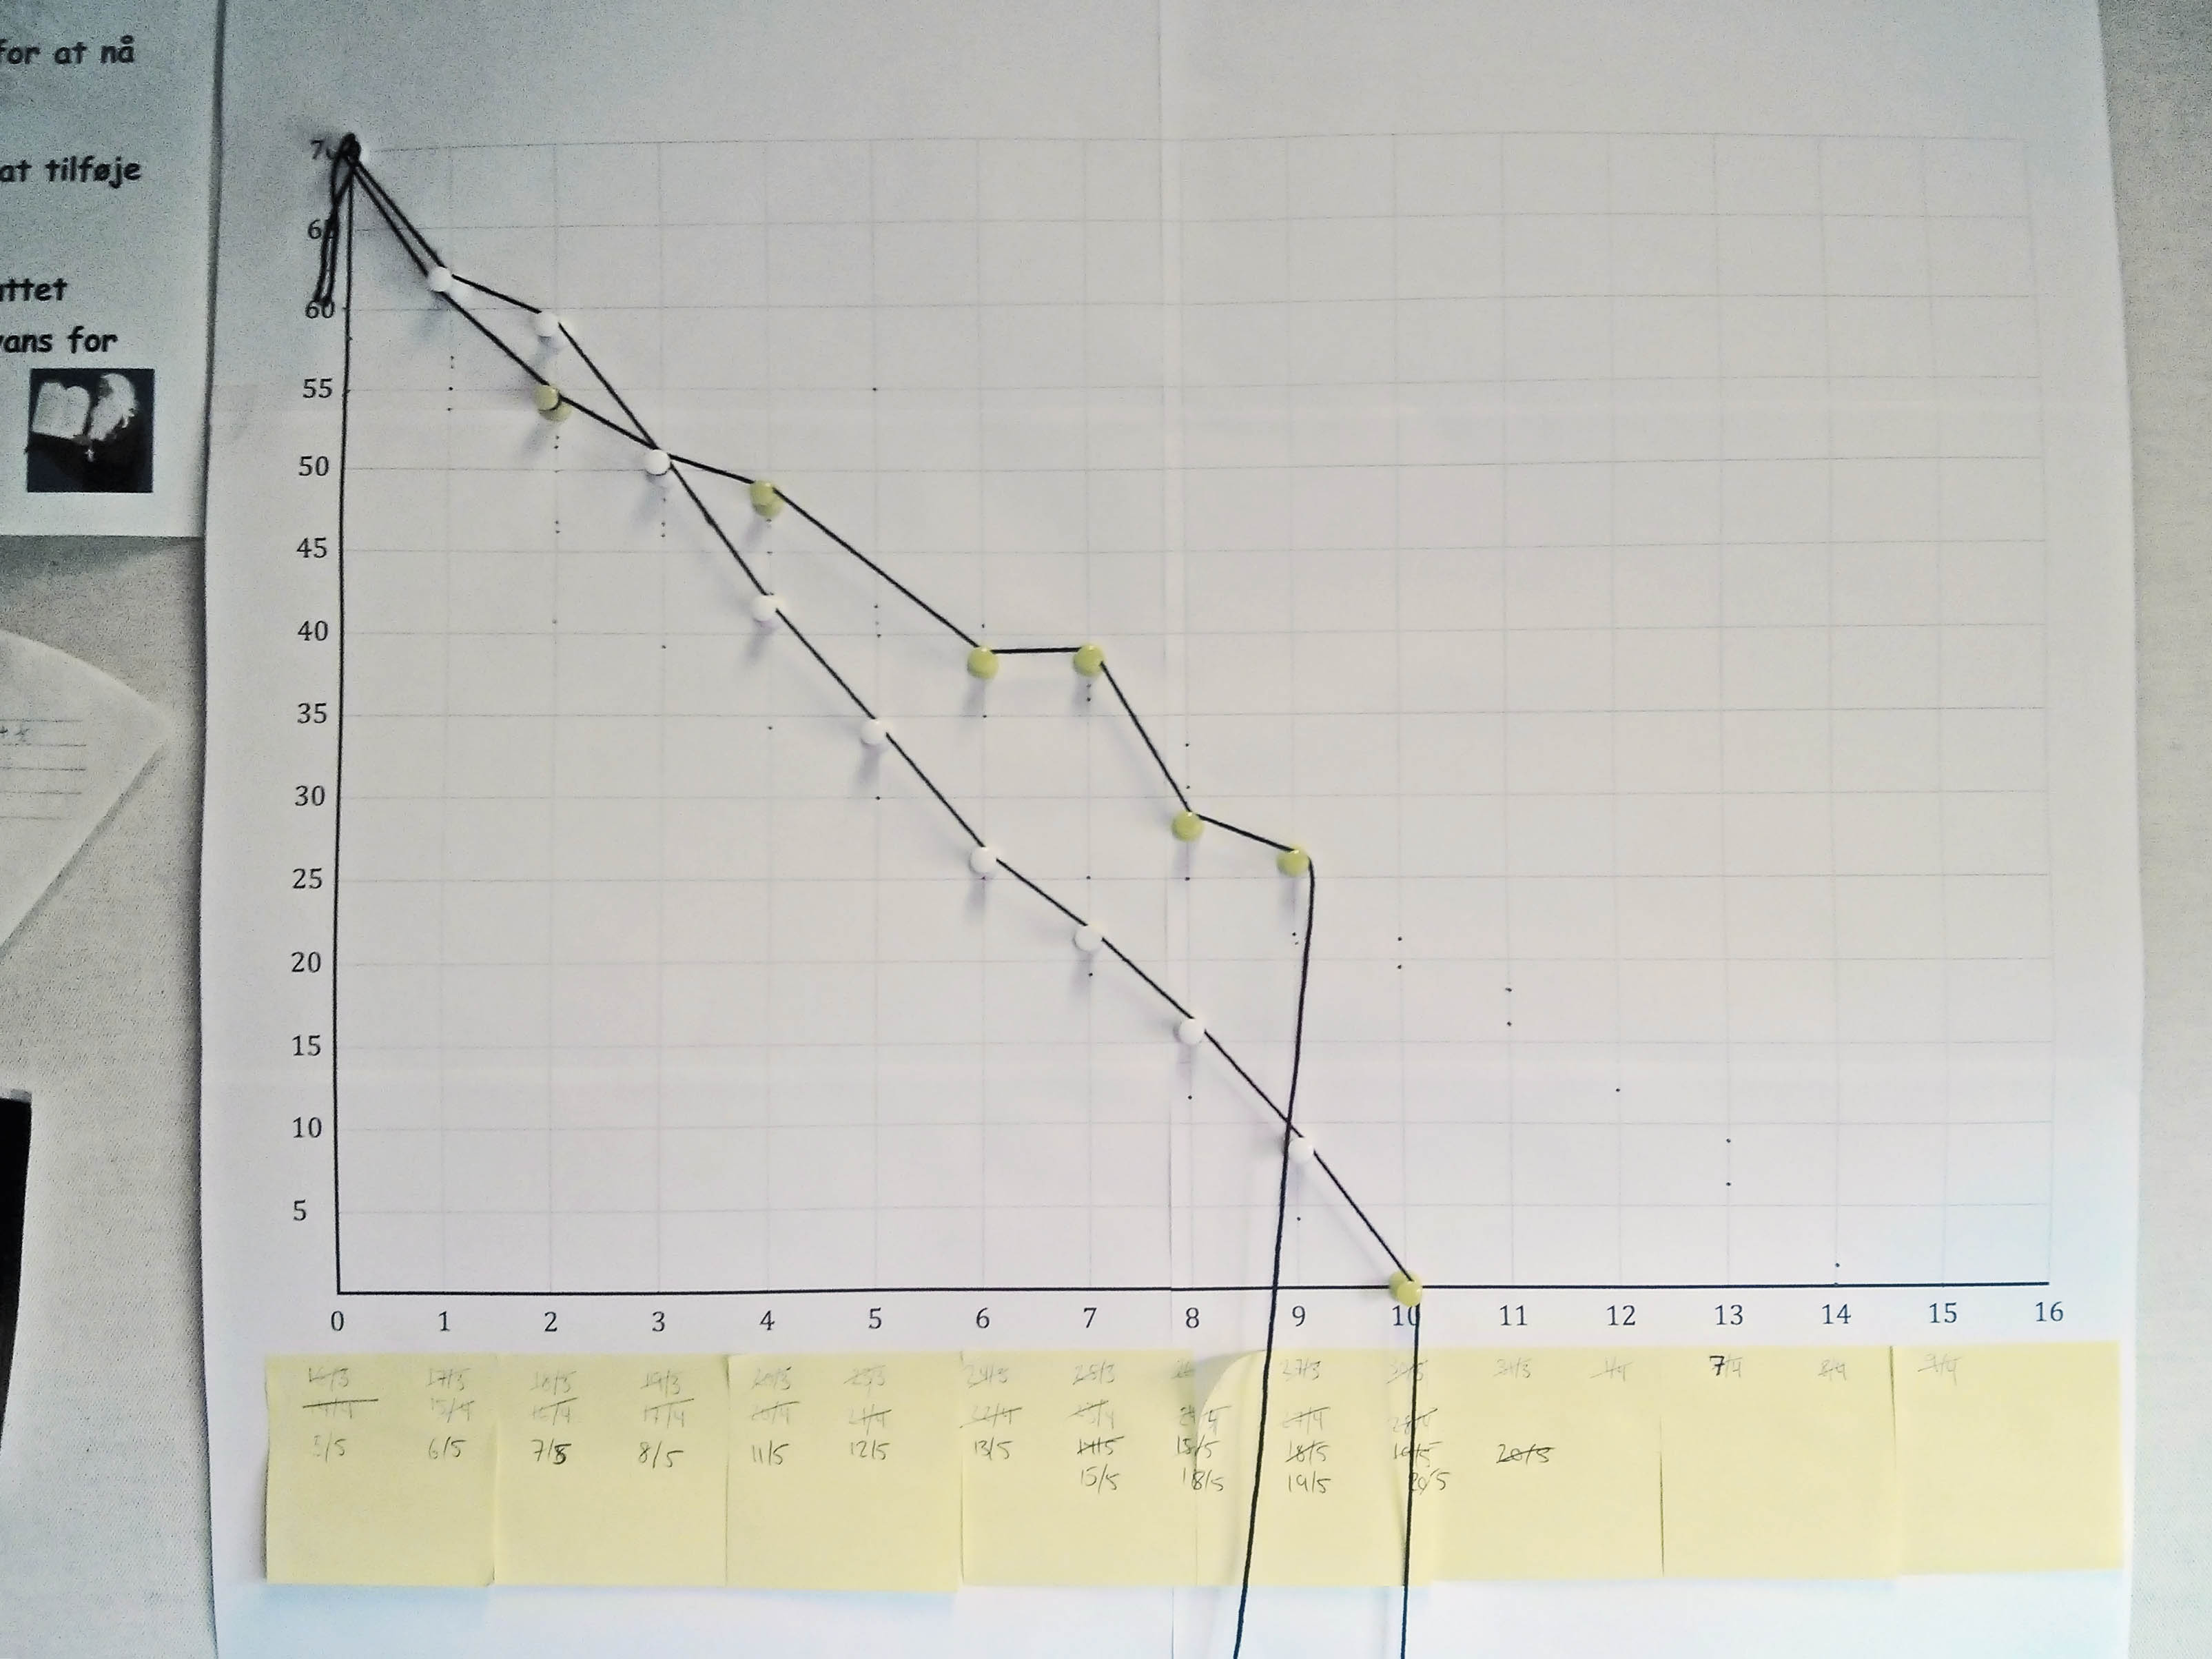
\includegraphics[width=0.49\textwidth]{burndown}~~~
    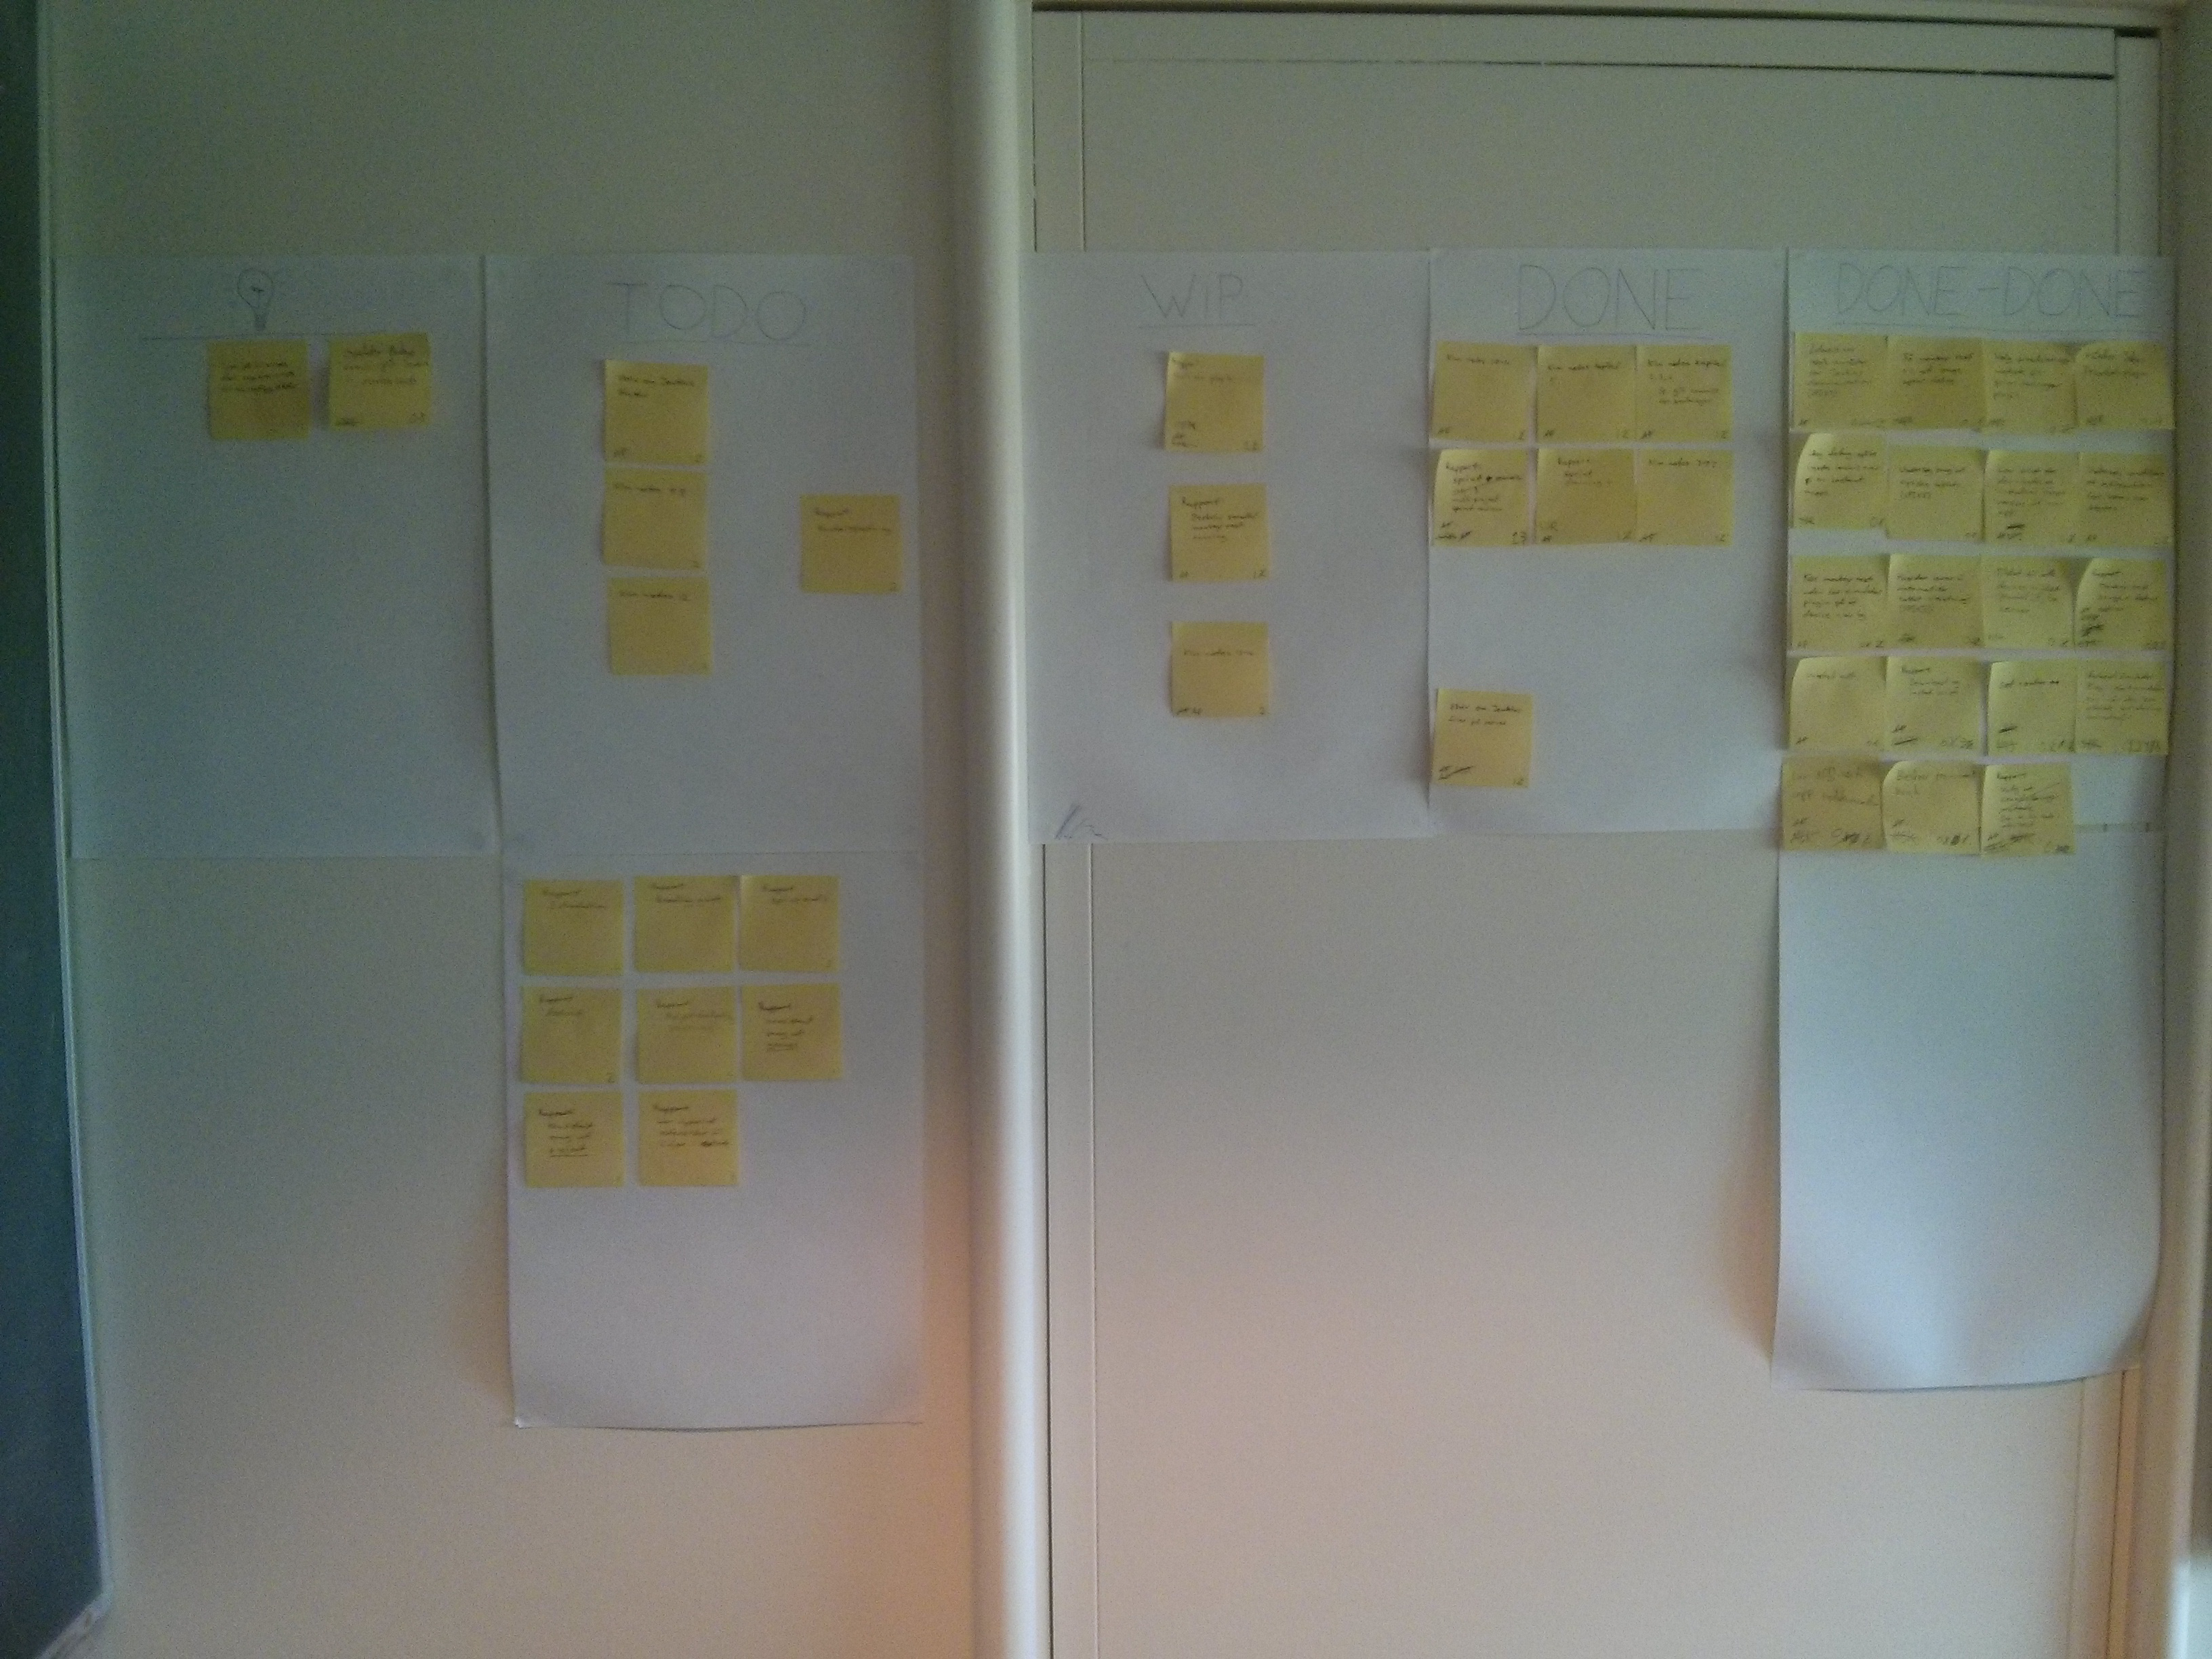
\includegraphics[width=0.49\textwidth]{kanban}

\end{frame}
\note{
	\begin{itemize}
		\item \textbf{Internt}: Valgt Scrum
    \item Det passer godt ind i multiprojektet.
    \item \textbf{Scrumboardet}: valgte backlog items > \textbf{opsplitning} i opgaver > \textbf{planning} poker. Enhed: \textbf{halvdage} (tidligere god erfaring)
    \item \textbf{Daily Scrum}
    \begin{itemize}
      \item Fortæller om \textbf{fremgang}, problemer, mm
      \item Vælger opgaver fra sprint backloggen
      \item Opdaterer \textbf{burndown}, visuel fremgang
    \end{itemize}

    \item På burndown: \textbf{Vi er bagefter}:
    \begin{itemize}
      \item Ideelle burndown, summerede resterende opgaver.
      \item \textbf{Prioriterer} resterende opgaver, \textbf{vigtigste fuldført}.
      \item Dette kan ses på scrumboardet. Nederste tasks er nedprioriterede.
    \end{itemize}
    
	\end{itemize}
}


%%%%%%%%%%%%%%%%%%%%%%%%%
%% SCM
%%%%%%%%%%%%%%%%%%%%%%%%%


\begin{frame}
    \frametitle{Continuous Integration}
    \begin{itemize}
      \item Hyppig merge med master branch
      \item Automatisk testning af apps og biblioteker
      \item Nyeste dokumentation
      \item Automatisk kørsel af statiske analyser
    \end{itemize}
\end{frame}
\note{
	\begin{itemize}
    \item \textbf{Agil}: giver \textbf{stort ansvar} til udviklerne.
    \item De \textbf{comitter direkte} til \textbf{master} branch, derfor skal de comitte \textbf{ofte}.
    \item Vi arbejder nemlig meget i de samme ting.
    \item[]
    \item Dette giver konstant \textbf{nye versioner}: skal konfig-styres.
    \item Tingene kan siges at blive\textbf{ understøttet af CI}.
	\end{itemize}
}